% -*- fill-column: 52 -*-
% (local-set-key (kbd "C-c C-f") 'display-fill-column-indicator-mode)
\chapter{Mélyvíz}
Most, hogy már tisztában vagyunk a Prolog
alapjaival, nézzük meg, hogy hogy néz ki egy
,,igazi'' Prolog program: az asszociációs struktúrát
megvalósító könyvtár \name{SWI-Prolog}ban.

Az alábbiakban bemutatott forráskódban nem
szerepelnek az \name{SWI-Prolog}-specifikus részek
és az angol nyelvű megjegyzések, de ettől (és
helyenként formázástól) eltekintve megegyezik az
eredetivel.

Mielőtt megnéznénk magát a programot, vizsgáljuk
meg, hogy mi is a probléma, amire megoldást ad, és
mi ennek az elméleti háttere.

\section{Asszociációs listák}
Programozáskor nagyon gyakran előfordul, hogy
adatokat \emph{kulcsokhoz} rendelünk, amelyek
szerint később ki akarjuk majd keresni őket. Az a
feltételezés, hogy különböző adatokhoz mindig
különböző kulcs tartozik. Ilyen kulcs lehet pl. egy
bankban a számlaszám, amihez a megfelelő számla
adatait rendelik. A kulcs-érték párokat tároló
adatstruktúrákat gyakran nevezik \emph{szótáraknak}
is, hiszen egy szótárban (enciklopédiában stb.) is
egy-egy címszóhoz vannak rendelve a
jelentések/magyarázatok.
\index{kulcs}\index{szotar@szótár}

A szótár legegyszerűbb megvalósítása az
\emph{asszociációs lista}, ahol a párokat egy
listában tároljuk: \index{asszociációs lista}
\begin{program}
empty_assoc([]).

put_assoc(K, A, V, [K-V|A]).

get_assoc(K, [K-V|_], V) :- !.
get_assoc(K, [K1-_|A], V) :-
    K \= K1, get_assoc(K, A, V).

del_assoc(K, [K-V|A], V, A1) :-
    !, del_assoc_others(K, A, A1).
del_assoc(K, [K1-V1|A], V, [K1-V1|A1]) :-
    K \= K1, del_assoc(K, A, V, A1).

del_assoc_others(_, [], []) :- !.
del_assoc_others(K, [K-_|A], A1) :-
    !, del_assoc_others(K, A, A1).
del_assoc_others(K, [K1-V1|A], [K1-V1|A1]) :-
    K \= K1, del_assoc_others(K, A, A1).
\end{program}
Itt az üres szótár egyszerűen egy üres lista; a
\pr{put\_assoc} egy asszociációs lista elejére rak
be egy kulcs-érték párt; a \pr{get\_assoc} megkeresi
a listában az első adott kulcsú értéket; a
\pr{del\_assoc} pedig kitörli ugyanezt. A törlésnél
figyelni kell arra, hogy az összes lehetséges
előfordulást töröljük, ezért ez mindig a teljes
listán végigmegy.

Amíg nincsen nagyon sok adatunk, ez a megoldás elég
jól működik. Az egyszerűségnek azonban ára van: mind
a keresés, mind a törlés általános esetben az elemek
számával arányos. Ezt úgy szokás megfogalmazni, hogy
a keresés és törlés komplexitása $O(n)$, ahol $n$ az
elemek száma. Ez az $O(n)$ (kiolvasva \emph{ordó
enn}) azt mondja, hogy nem biztos, hogy pontosan $n$
művelet, lehet hogy $n+2$, vagy $5n$, de ha az
$n$-et 100-szor akkorára választom, akkor a
műveletigény is körülbelül 100-szor akkorára
nő. (Egy $O(n^2)$-es algoritmus esetén ilyenkor a
műveletigény kb.~a 10 000-szeresére változna.)
\index{ordó}\index{komplexitás}

A következőkben bemutatott módszer olyan, hogy
mindhárom művelet (beszúrás, keresés, törlés)
egyaránt $O(\log n)$ komplexitású, tehát ha az $n$ a
100-szorosára nő, akkor a műveletigény
kb.~6--7-szeresére változik. A beszúrás a fenti
egyszerű verzióban gyorsabb -- $O(1)$ --, de a
keresés és törlés hatékonysága miatt érdemesebb az
alábbi adatstruktúrákat alkalmazni.

\section{Bináris keresőfák}
Tegyük fel, hogy a kulcsok sorbarendezhetőek
(Prologban tetszőleges két kifejezés sorbarendezhető
a \pr{@<} operátorral). Ekkor a kulcsokat egy olyan
(általában fejjel lefele ábrázolt) fa alakú
struktúrába lehet szervezni, ami mindig legfeljebb
kétfelé ágazik el (ezért \emph{bináris fának}
hívják). Nézzünk egy példát, ahol a kulcsok számok:
\index{\pr{"@<}}\index{fa!bináris}

\begin{center}
\begin{tikzpicture}[level distance=1cm,
    level 1/.style={sibling distance=3cm},
    level 2/.style={sibling distance=1.5cm}]
  \node {8}
  child {
    node {3}
    child { node {1} }
    child {
      node {6}
      child { node {4} }
      child { node {7} }
    }
  }
  child {
    node {10}
    child { edge from parent[draw=none] }
    child {
      node {14}
      child { node {13} }
      child { edge from parent[draw=none] }
    }
  };
\end{tikzpicture}
\end{center}
Itt a fa \emph{gyökere} a 8, belső \emph{csúcsok} a
3, 10, 6 és 14, és a fa \emph{levelei} az 1, 4, 7 és
13. Amikor egy csúcsból csak egy ág megy tovább
(pl.~10, 14), olyankor is az ág vagy balra, vagy
jobbra megy. Egy ilyen fát könnyen le tudunk írni
Prologban, például egy \pr{fa} struktúrával, aminek
az első argumentuma a kulcs, a második és harmadik
pedig a bal- és jobboldali ág (a nem létező ágakat
jelölje mondjuk a \pr{-}):
\begin{program}
fa(8, fa(3, fa(1, -, -),
            fa(6, fa(4, -, -),
                  fa(7, -, -))),
      fa(10, -,
             fa(14, fa(13, -, -),
                    -)))
\end{program}
(Egy másik lehetőség, hogy a levelekre egy külön
\pr{levél} funktort használunk stb.)

A fenti példában szereplő fának van egy különleges
tulajdonsága: egy csúcs alatti baloldali ágon (és az
abból kijövő ágakon stb.) minden elem kisebb, a
jobboldali ágon pedig mindegyik nagyobb, mint a
csúcsban levő érték. Az ilyen tulajdonságú fákat
\emph{keresőfának} nevezik.
\index{fa!kereső-}

Ha meg akarunk keresni egy elemet, akkor elindulunk
a gyökértől, és aszerint, hogy a keresett kulcs
kisebb, vagy nagyobb, balra ill. jobbra megyünk
tovább. Ezt addig folytatjuk, amíg meg nem találjuk
a keresett elemet, vagy egy levélhez nem érünk. A
keresés műveletigénye tehát a fa magasságával
arányos. A beszúrásról és törlésről hasonlóan
megmutatható, hogy a fa magasságától függ a
komplexitásuk. Ha az adatok szépen egyenletesen
helyezkednek el, akkor ez hozzávetőlegesen $\log n$
lesz (2-es alapú logaritmussal).

Sajnos azonban ez nem feltétlenül teljesül -- pl.~ez
is egy keresőfa:

\begin{center}
\begin{tikzpicture}[level distance=1cm]
  \node {5}
  child {
    node {4}
    child {
      node {3}
      child {
        node {2}
        child { node {1} }
        child { edge from parent[draw=none] }
      }
      child { edge from parent[draw=none] }
    }
    child { edge from parent[draw=none] }
  }
  child { edge from parent[draw=none] };
\end{tikzpicture}
\end{center}
\dots de itt a fa magassága az elemek számával
azonos.

\section{AVL-fák}
Egy lehetséges megoldása ennek a problémának az,
hogy megköveteljük, hogy a fa mindig
\emph{kiegyensúlyozott} legyen, tehát minden
csúcsnál a bal- és jobb ághoz tartozó részfa
magassága legfeljebb 1-el különbözhet. A fenti
példában a 8-as alatti két részfa magassága egyaránt
3, a 3-as alatti két részfa magassága 1 és 2, de
pl.~a 10-es alatti két részfa magassága 0 és 2,
tehát ez nem kiegyensúlyozott. Ha a 10-14-13 hármast
,,átforgatjuk'', akkor kiegyensúlyozottá válik:
\index{fa!kiegyensúlyozott}

\begin{center}
\begin{tikzpicture}[level distance=1cm,
    level 1/.style={sibling distance=3cm},
    level 2/.style={sibling distance=1.5cm}]
  \node {8}
  child {
    node {3}
    child { node {1} }
    child {
      node {6}
      child { node {4} }
      child { node {7} }
    }
  }
  child {
    node {13}
    child { node {10} }
    child { node {14} }
  };
\end{tikzpicture}
\end{center}
A beszúrás és törlés műveletekbe ilyen jellegű
forgatásokat épít be az \emph{AVL-fa}, hogy
biztosítja a kiegyensúlyozottságot. Ezt a módszert
1962-ben publikálta két szovjet matematikus,
Adelszon-Velszkij és Landisz, az ő vezetéknevükből
származik az adastruktúra elnevezése.
\index{fa!AVL-}

\begin{infobox}{}{asszociatív tárolók}
Egy másik, kicsit bonyolultabb keresőfa a
\emph{piros-fekete fa}, ami az egyes elemekhez
(piros vagy fekete) színt rendel, és ennek
segítségével még hatékonyabb beszúrást/törlést tesz
lehetővé, mint az AVL-fa. Cserébe viszont a keresés
egy kicsit lassabb lehet.
\index{fa!piros-fekete}

A kulcs szerinti keresés problémájára még egy nagyon
érdekes megoldást adnak a \emph{hash táblák},
melyeknek rengeteg variánsa létezik. Ezek általában
sokkal gyorsabbak, mint a keresőfák ($O(1)$
átlagosan), de időnként lassabbak is lehetnek
($O(n)$ legrosszabb esetben), valamint az elemeket
nem rendezetten tárolják.
\index{hash tábla}

Prologban nincs mód egy adat
\emph{megváltoztatására}, csak egy módosított
változat készítésére (tehát az adatok
\emph{perzisztensek}).\index{perzisztencia} Ilyen
megkötések mellett a hatékonysághoz időnként trükkök
kellenek -- erről szól Chris Okasaki
könyve,\footnote[2]{Ch.~Okasaki, \emph{Purely
  Functional Data Structures}, Cambridge, 1996.}
nagyon érdekes olvasmány.
\end{infobox}

Az alább vizsgált program AVL-fát használ a szótár
megvalósítására -- a pontos részleteket majd
útközben megbeszéljük. Kalandra fel!

\section{A program}
{\scriptsize
\begin{program}
/*  Part of SWI-Prolog

    Author:        R.A.O'Keefe, L.Damas, V.S.Costa, Glenn Burgess,
                   Jiri Spitz and Jan Wielemaker
    E-mail:        J.Wielemaker@vu.nl
    WWW:           http://www.swi-prolog.org
    Copyright (c)  2004-2018, various people and institutions
    All rights reserved.

    Redistribution and use in source and binary forms, with or without
    modification, are permitted provided that the following conditions
    are met:

    1. Redistributions of source code must retain the above copyright
       notice, this list of conditions and the following disclaimer.

    2. Redistributions in binary form must reproduce the above copyright
       notice, this list of conditions and the following disclaimer in
       the documentation and/or other materials provided with the
       distribution.

    THIS SOFTWARE IS PROVIDED BY THE COPYRIGHT HOLDERS AND CONTRIBUTORS
    "AS IS" AND ANY EXPRESS OR IMPLIED WARRANTIES, INCLUDING, BUT NOT
    LIMITED TO, THE IMPLIED WARRANTIES OF MERCHANTABILITY AND FITNESS
    FOR A PARTICULAR PURPOSE ARE DISCLAIMED. IN NO EVENT SHALL THE
    COPYRIGHT OWNER OR CONTRIBUTORS BE LIABLE FOR ANY DIRECT, INDIRECT,
    INCIDENTAL, SPECIAL, EXEMPLARY, OR CONSEQUENTIAL DAMAGES (INCLUDING,
    BUT NOT LIMITED TO, PROCUREMENT OF SUBSTITUTE GOODS OR SERVICES;
    LOSS OF USE, DATA, OR PROFITS; OR BUSINESS INTERRUPTION) HOWEVER
    CAUSED AND ON ANY THEORY OF LIABILITY, WHETHER IN CONTRACT, STRICT
    LIABILITY, OR TORT (INCLUDING NEGLIGENCE OR OTHERWISE) ARISING IN
    ANY WAY OUT OF THE USE OF THIS SOFTWARE, EVEN IF ADVISED OF THE
    POSSIBILITY OF SUCH DAMAGE.
*/
\end{program}
}\noindent%
Ez (szó szerint) a ,,kisbetűs rész''. A programok
elején szokás felsorolni a szerzőket, illetve
meghatározni, hogy a program milyen feltételekkel
terjeszthető. A \pr{/*} és \pr{*/} közti rész
megjegyzésnek számít, olyan, mint ha minden sor
elején lenne egy \pr{\%}
szimbólum.\index{\pr{/*\dots*/}}

%% {\footnotesize\begin{program*}
%% :- module(assoc,
%%      [ empty_assoc/1,       % -Assoc
%%        is_assoc/1,          % +Assoc
%%        assoc_to_list/2,     % +Assoc, -Pairs
%%        assoc_to_keys/2,     % +Assoc, -List
%%        assoc_to_values/2,   % +Assoc, -List
%%        gen_assoc/3,         % ?Key, +Assoc, ?Value
%%        get_assoc/3,         % +Key, +Assoc, ?Value
%%        get_assoc/5,         % +Key, +Assoc0, ?Val0, ?Assoc, ?Val
%%        list_to_assoc/2,     % +List, ?Assoc
%%        map_assoc/2,         % :Goal, +Assoc
%%        map_assoc/3,         % :Goal, +Assoc0, ?Assoc
%%        max_assoc/3,         % +Assoc, ?Key, ?Value
%%        min_assoc/3,         % +Assoc, ?Key, ?Value
%%        ord_list_to_assoc/2, % +List, ?Assoc
%%        put_assoc/4,         % +Key, +Assoc0, +Value, ?Assoc
%%        del_assoc/4,         % +Key, +Assoc0, ?Value, ?Assoc
%%        del_min_assoc/4,     % +Assoc0, ?Key, ?Value, ?Assoc
%%        del_max_assoc/4      % +Assoc0, ?Key, ?Value, ?Assoc
%%      ]).
%% \end{program*}
%% }\noindent%

Mielőtt rátérnénk a lényegre, érdemes még pár szót
ejteni a \emph{modulok}\/ról.  Prologban a
programokat könyvtárakba vagy modulokba lehet
szervezni. Ezek megadásának módja nem szerepelt az
eredeti ISO-szabványban, és bár egy későbbi
kiegészítésbe belekerült, ezt kevés Prolog rendszer
követi, mindegyik kicsit máshogyan működik.
\index{modul}\index{konyvtar@könyvtár}

A modulok mindig tartalmaznak egy listát azon
\emph{exportált} szabályokról, amelyek ,,kívülről''
(más programfájlokból) is látszanak. Ezzel el lehet
rejteni azokat a szabályokat, amelyek nem tartoznak
hozzá a könyvtár lényegi funkcióihoz (az
\emph{interfész}\/hez). A fenti kezdetleges
asszociációs listánknál például a
\pr{del\_assoc\_others} volt egy ilyen lokális
szabály, amit a \pr{del\_assoc} ugyan használ, de a
könyvtárat használó más program már jobb, ha nem
lát.  \index{exportálás}\index{interfész}

A kompatibilitás kedvéért a modul definícióját
kihagyjuk, de az alábbiakban az exportált szabályok
könnyen felismerhetőek lesznek az őket megelőző
megjegyzésről, ahogy máris látni fogjuk.

\begin{program*}
% empty_assoc(?Assoc) [semidet]
empty_assoc(t).
\end{program*}
A \emph{semidet} egyike a szabályok öt lehetséges
kategóriájának:
\begin{itemize}
\item \emph{det} (determinisztikus): mindig pontosan
  egyszer teljesül, pl.~\pr{összeg(+L, -Ö)}
\item \emph{semidet} (félig determinisztikus):
  legfeljebb egyszer teljesül, pl.~\pr{maximum(+L,
    -M)} [üres listára sikertelen]
\item \emph{multi} (többszörös): legalább egyszer
  teljesül, pl.~\pr{permutáció(+L, -P)}
\item \emph{nondet} (nemdeterminisztikus): többször
  teljesülhet, de lehet sikertelen is,
  pl.~\pr{tartalmaz(?E, ?L)}
\item \emph{failure} (sikertelen): sosem teljesül,
  pl.~\pr{fail}
\end{itemize}
\index{determinisztikusság}
Ezeket mind úgy kell érteni, hogy ,,ha a
dokumentációjának megfelelően adjuk meg a
paramétereket''.

Visszatérve az AVL-fára, az üres fát itt a \pr{t}
atom fogja jelölni (nem a \pr{-}, mint fent a
bináris fánál).

\begin{program*}
% assoc_to_list(+Assoc, -Pairs) [det]
assoc_to_list(Assoc, List) :-
    assoc_to_list(Assoc, List, []).

assoc_to_list(t(Key,Val,_,L,R), List, Rest) :-
    assoc_to_list(L, List, [Key-Val|More]),
    assoc_to_list(R, More, Rest).
assoc_to_list(t, List, List).
\end{program*}
Az \pr{assoc\_to\_list} szabály egy AVL-fából párok
listáját hozza létre. Akkumulátoros megoldás
(ld.~6.~lecke), tehát egy üres akkumulátor
paraméterrel meghívja a 3-argumentumú változatot. Az
AVL-fa egy csúcsát a \pr{t(K,V,B,L,R)} struktúra
írja le, ahol \pr{K} és \pr{V} a kulcs és a hozzá
tartozó érték, \pr{B} a kiegyensúlyozáshoz használt
szimbólum (\pr{-} ha a két részfa azonos magasságú,
\pr{<} ill.~\pr{>} ha a baloldali ill. jobboldali
magasabb), \pr{L} és \pr{R} pedig a bal- és
jobboldali részfa.

\begin{program*}
% assoc_to_keys(+Assoc, -Keys) [det]
assoc_to_keys(Assoc, List) :-
    assoc_to_keys(Assoc, List, []).

assoc_to_keys(t(Key,_,_,L,R), List, Rest) :-
    assoc_to_keys(L, List, [Key|More]),
    assoc_to_keys(R, More, Rest).
assoc_to_keys(t, List, List).

% assoc_to_values(+Assoc, -Values) [det]
assoc_to_values(Assoc, List) :-
    assoc_to_values(Assoc, List, []).

assoc_to_values(t(_,Value,_,L,R), List, Rest) :-
    assoc_to_values(L, List, [Value|More]),
    assoc_to_values(R, More, Rest).
assoc_to_values(t, List, List).
\end{program*}
Ez a két szabály gyakorlatilag ugyanaz, mint az
előző, csak nem kulcs-érték párokat gyűjtenek ki
listába, hanem rendre kulcsokat illetve értékeket.

\begin{program*}
% is_assoc(+Assoc) [semidet]
is_assoc(Assoc) :-
    is_assoc(Assoc, _Min, _Max, _Depth).

is_assoc(t,X,X,0) :- !.
is_assoc(t(K,_,-,t,t),K,K,1) :- !, ground(K).
is_assoc(t(K,_,>,t,t(RK,_,-,t,t)),K,RK,2) :-
    !, ground((K,RK)), K @< RK.

is_assoc(t(K,_,<,t(LK,_,-,t,t),t),LK,K,2) :-
    !, ground((LK,K)), LK @< K.

is_assoc(t(K,_,B,L,R),Min,Max,Depth) :-
    is_assoc(L,Min,LMax,LDepth),
    is_assoc(R,RMin,Max,RDepth),
    compare(Rel,RDepth,LDepth),
    balance(Rel,B),
    ground((LMax,K,RMin)),
    LMax @< K,
    K @< RMin,
    Depth is max(LDepth, RDepth)+1.

balance(=,-).
balance(<,<).
balance(>,>).
\end{program*}
Az \pr{is\_assoc} ellenőrzi, hogy a paraméterben
kapott kifejezés egy helyes AVL-fa-e. Az első
szabály csak meghívja a 4-argumentumú verziót. A
többi az 5 lehetséges esetet kezeli:
\begin{enumerate}
\item Az \emph{üres fa} egy helyes AVL-fa. (A többi
  paraméter értéke itt érdektelen, de azért valami
  értelmesre vannak beállítva.)
\item A \emph{levél} minimuma és maximuma is a
  levélben szereplő kulcs, a mélysége pedig 1. A
  \pr{ground} azt ellenőrzi, hogy a kulcsban nem
  szerepel ismeretlen változó. (Ez nem teljesen
  szabványos, de a gyakorlatban minden Prolog
  implementáció támogatja.)\index{\pr{ground}}
\item Ha csak a \emph{baloldali részfa üres}, a
  jobboldali részfa alatti részfák üresek kell, hogy
  legyenek, és az egész fa mélysége 2. Ellenőrzi,
  hogy a kulcsokban nincsenek ismeretlenek, és a
  jobboldali részfa kulcsa nagyobb, mint a gyökéré.
\item Ha csak a \emph{jobboldali részfa üres}, akkor
  ugyanez fordítva.
\item Ha \emph{egyik részfa sem üres}, akkor
  rekurzívan ellenőrzi mindkettőt. A fa minimuma a
  baloldali részfa minimuma, a maximuma pedig a
  jobboldali részfa maximuma lesz. A részfák
  mélységét összehasonlítja a \pr{compare}
  segítségével (szintén egy csak \emph{de facto}
  szabványos szabály), ami az első argumentumban
  \pr{<}, \pr{=} vagy \pr{>} lesz. Ellenőrzi, hogy
  ennek megfelel-e a fában szereplő \pr{B} szimbólum
  (a \pr{balance} az \pr{=} jelből \pr{-} jelet
  csinál), és hogy a kulcs a baloldali maximum és a
  jobboldali minimum közé esik. A mélység eggyel
  több, mint a két részfa mélysége közül a
  nagyobbik.\index{\pr{compare}}
\end{enumerate}

\begin{program*}
% gen_assoc(?Key, +Assoc, ?Value) [nondet]
gen_assoc(Key, Assoc, Value) :-
    (   ground(Key)
    ->  get_assoc(Key, Assoc, Value)
    ;   gen_assoc_(Key, Assoc, Value)
    ).

gen_assoc_(Key, t(_,_,_,L,_), Val) :-
    gen_assoc_(Key, L, Val).
gen_assoc_(Key, t(Key,Val,_,_,_), Val).
gen_assoc_(Key, t(_,_,_,_,R), Val) :-
    gen_assoc_(Key, R, Val).
\end{program*}
A \pr{gen\_assoc} egy olyan keresés, ami fordítva is
tud működni: meg tud keresni egy adott értékhez
tartozó kulcsot (természetesen ez nem lesz
hatékony), vagy ha az érték sincsen megadva, akkor
végigmegy az összes kulcs-érték páron. Ha a kulcs
meg van adva, akkor ugyanazt csinálja, mint a
\pr{get\_assoc}.

Mivel először a baloldali részfát vizsgálja, utána a
gyökérben levő értéket, és végül a jobboldali
részfát (\emph{infix} bejárás), a kulcsokat növekvő
sorrendben fogja végigvenni.

\begin{program*}
% get_assoc(+Key, +Assoc, -Value) [semidet]
get_assoc(Key, t(K,V,_,L,R), Val) :-
    compare(Rel, Key, K),
    get_assoc(Rel, Key, V, L, R, Val).

get_assoc(=, _, Val, _, _, Val).
get_assoc(<, Key, _, Tree, _, Val) :-
    get_assoc(Key, Tree, Val).
get_assoc(>, Key, _, _, Tree, Val) :-
    get_assoc(Key, Tree, Val).
\end{program*}
Megadott kulcs alapján keres.
\begin{program*}
% get_assoc(+Key, +Assoc0, ?Val0, ?Assoc, ?Val)
%                                         [semidet]
get_assoc(Key, t(K,V,B,L,R), Val,
          t(K,NV,B,NL,NR), NVal) :-
    compare(Rel, Key, K),
    get_assoc(Rel, Key, V, L, R, Val,
              NV, NL, NR, NVal).

get_assoc(=, _, Val, L, R, Val, NVal, L, R, NVal).
get_assoc(<, Key, V, L, R, Val, V, NL, R, NVal) :-
    get_assoc(Key, L, Val, NL, NVal).
get_assoc(>, Key, V, L, R, Val, V, L, NR, NVal) :-
    get_assoc(Key, R, Val, NR, NVal).
\end{program*}
Ez a változat arra használható, hogy egy már létező
kulcshoz tartozó értéket lecseréljünk. A harmadik
argumentum a kulcshoz tartozó régi érték, a negyedik
az így keletkező AVL-fa, és az utolsó az új érték.

\begin{program*}
% list_to_assoc(+Pairs, -Assoc) [det]
list_to_assoc(List, Assoc) :-
    (  List = [] -> Assoc = t
    ;  keysort(List, Sorted),
       length(Sorted, N),
       list_to_assoc(N, Sorted, [], _, Assoc)
    ).

list_to_assoc(1, [K-V|More], More,
              1, t(K,V,-,t,t)) :- !.
list_to_assoc(2, [K1-V1,K2-V2|More], More,
              2, t(K2,V2,<,t(K1,V1,-,t,t),t)) :- !.
list_to_assoc(N, List, More,
              Depth, t(K,V,Balance,L,R)) :-
    N0 is N - 1,
    RN is N0 div 2,
    Rem is N0 mod 2,
    LN is RN + Rem,
    list_to_assoc(LN, List, [K-V|Upper], LDepth, L),
    list_to_assoc(RN, Upper, More, RDepth, R),
    Depth is LDepth + 1,
    compare(B, RDepth, LDepth), balance(B, Balance).
\end{program*}
Az \pr{assoc\_to\_list} fordítottja. A fa hatékony
építéséhez először sorbarakja az elemeket a kulcsok
szerint a \pr{keysort} szabály segítségével. (Ez
megint egy nem teljesen szabványos, de általánosan
elfogadott szabály -- szükség esetén könnyen
megírható az összefűzéses keresés mintájára. Ugyanez
igaz a \pr{length}re, amit mi \pr{hossz} néven
definiáltunk.)
\index{\pr{keysort}}\index{\pr{length}}

A fa építését az 5-argumentumú verzió végzi. Az első
argumentum az elemek száma, a második és harmadik
elem együtt a rendezett elemek különbség-listája, a
negyedik a fa mélysége, és az utolsó a készített
AVL-fa. Az elemek száma alapján:
\begin{enumerate}
\item Ha \emph{1 elem van}, akkor egy 1 mélységű,
  egy levélből álló fa az eredmény.
\item Ha \emph{2 elem van}, akkor egy 2 mélységű,
  egy bal-levéllel rendelkező fa az eredmény.
\item Ha \emph{legalább 3 elem van}, akkor
  rekurzívan elkészít két részfát, amelyek a lista
  első ill.~második felét tartalmazzák. Kicsit
  pontosabban, a két részfa összesen $n-1$
  elemet tárol (mivel 1 a gyökérbe kerül), és ha ez
  nem páros, akkor a baloldaliban lesz több elem. A
  különbség-lista itt lesz hasznos: az első \pr{LN}
  elemből elkészül az \pr{L} fa, és a \pr{List}
  listából fel nem használt maradékot a
  \pr{[K-V|Upper]} listával egyesíti. Ezáltal a
  gyökérhez tartozó kulcs-érték pár és a jobboldali
  fa építéséhez szükséges \pr{Upper} lista is rögtön
  adott. Mivel a baloldali részfában van több elem,
  a mélység eggyel több lesz, mint a baloldali
  mélység. Végül a bal- és jobb mélység alapján
  kiszámolja a gyökérhez tartozó \pr{B} értéket
  (\pr{<}, \pr{-} vagy \pr{>}).
\end{enumerate}

\begin{program*}
% ord_list_to_assoc(+Pairs, -Assoc) [det]
ord_list_to_assoc(Sorted, Assoc) :-
    (  Sorted = [] -> Assoc = t
    ;  length(Sorted, N),
       list_to_assoc(N, Sorted, [], _, Assoc)
    ).
\end{program*}
Ugyanez, csak már feltételezi, hogy a lista elemei
rendezettek.

\begin{program*}
% map_assoc(:Pred, +Assoc) [semidet]
map_assoc(Pred, T) :-
    map_assoc_(T, Pred).

map_assoc_(t, _).
map_assoc_(t(_,Val,_,L,R), Pred) :-
    map_assoc_(L, Pred),
    call(Pred, Val),
    map_assoc_(R, Pred).
\end{program*}
Infix bejárással végigmegy az elemeken, és
mindegyikre meghívja az első argumentumban kapott
szabályt.

\begin{program*}
% map_assoc(:Pred, +Assoc0, ?Assoc) [semidet]
map_assoc(Pred, T0, T) :-
    map_assoc_(T0, Pred, T).

map_assoc_(t, _, t).
map_assoc_(t(Key,Val,B,L0,R0), Pred,
           t(Key,Ans,B,L1,R1)) :-
    map_assoc_(L0, Pred, L1),
    call(Pred, Val, Ans),
    map_assoc_(R0, Pred, R1).
\end{program*}
Ez a változat két argumentumot ad a kapott
szabályhoz: az első (\pr{Val}) az éppen vizsgált
érték, mint az előző verzióban, a második (\pr{Ans})
pedig egy változó, amire az adott elemet lecserélve
egy új fát épít. Ezzel tehát lehet olyat csinálni,
hogy minden értéket a fában négyzetre emelünk stb.

\begin{program*}
% max_assoc(+Assoc, -Key, -Value) [semidet]
max_assoc(t(K,V,_,_,R), Key, Val) :-
    max_assoc(R, K, V, Key, Val).

max_assoc(t, K, V, K, V).
max_assoc(t(K,V,_,_,R), _, _, Key, Val) :-
    max_assoc(R, K, V, Key, Val).
\end{program*}
Megkeresi a legnagyobb kulcsot a fában, és a hozzá
tartozó értéket.

\begin{program*}
% min_assoc(+Assoc, -Key, -Value) [semidet]
min_assoc(t(K,V,_,L,_), Key, Val) :-
    min_assoc(L, K, V, Key, Val).

min_assoc(t, K, V, K, V).
min_assoc(t(K,V,_,L,_), _, _, Key, Val) :-
    min_assoc(L, K, V, Key, Val).
\end{program*}
Ugyanez a legkisebb kulcsra.

\begin{program*}
% put_assoc(+Key, +Assoc0, +Value, -Assoc) [det]
put_assoc(Key, A0, Value, A) :-
    insert(A0, Key, Value, A, _).

insert(t, Key, Val, t(Key,Val,-,t,t), yes).
insert(t(Key,Val,B,L,R), K, V,
       NewTree, WhatHasChanged) :-
    compare(Rel, K, Key),
    insert(Rel, t(Key,Val,B,L,R), K, V,
           NewTree, WhatHasChanged).

insert(=, t(Key,_,B,L,R), _, V, t(Key,V,B,L,R), no).
insert(<, t(Key,Val,B,L,R), K, V,
       NewTree, WhatHasChanged) :-
    insert(L, K, V, NewL, LeftHasChanged),
    adjust(LeftHasChanged, t(Key,Val,B,NewL,R),
           left, NewTree, WhatHasChanged).
insert(>, t(Key,Val,B,L,R), K, V,
       NewTree, WhatHasChanged) :-
    insert(R, K, V, NewR, RightHasChanged),
    adjust(RightHasChanged, t(Key,Val,B,L,NewR),
           right, NewTree, WhatHasChanged).
\end{program*}
A beszúrásnál először az \pr{insert/5} szabály
hívódik meg, aminek utolsó argumentuma azt mondja
meg, hogy nőtt-e a fa mélysége. Ez az üres fa esetét
lekezeli, egyébként pedig a felelősséget az
\pr{insert/6} szabályra hárítja. Ennek az
argumentumai:
\begin{enumerate}
\item A gyökérben levő kulcs hogyan viszonyul a
  beszúrandó kulcshoz (\pr{<}, \pr{=}, \pr{>}).
\item Az eredeti AVL-fa.
\item A beszúrandó kulcs.
\item A beszúrandó érték.
\item Az új AVL-fa.
\item Nőtt-e a fa mélysége.
\end{enumerate}

Ha a kulcsok megegyeznek, akkor a hozzá tartozó
értéket a megadottra lecseréli. Ha a beszúrandó
kulcs a kisebb, akkor a baloldali részfán végez
rekurzívan beszúrást (az \pr{insert/5}-tel), majd az
\pr{adjust} szabállyal (ld. lent) biztosítja a
kiegyensúlyozottságot; ha a beszúrandó kulcs a
nagyobb, akkor ugyanez a jobboldali részfával.

\begin{program*}
adjust(no, Oldree, _, Oldree, no).
adjust(yes, t(Key,Val,B0,L,R), LoR,
       NewTree, WhatHasChanged) :-
    table(B0, LoR, B1,
          WhatHasChanged, ToBeRebalanced),
    rebalance(ToBeRebalanced, t(Key,Val,B0,L,R), B1,
              NewTree, _, _).

table(-, left , <, yes, no ) :- !.
table(-, right, >, yes, no ) :- !.
table(<, left , -, no , yes) :- !.
table(<, right, -, no , no ) :- !.
table(>, left , -, no , no ) :- !.
table(>, right, -, no , yes) :- !.
\end{program*}
Az \pr{adjust} első argumentuma, hogy történt-e
beszúrás. Ha nem, akkor a kulcsok változatlanok,
tehát a kiegyensúlyozottság továbbra is teljesül. A
második argumentum a módosított AVL-fa, a harmadik
azt mondja meg, hogy a bal vagy jobb részfát
módosítottuk (\pr{left} ill.~\pr{right}), a negyedik
a kiegyensúlyozás után kapott AVL-fa, az utolsó
pedig azt jelzi, hogy nőtt-e a fa mélysége.

A \pr{table} táblázatból könnyen kiolvasható, hogy a
6 lehetséges esetben mi történik: mi lesz az új
egyensúly-szimbólum (\pr{<}, \pr{-} vagy \pr{>}),
megnövekedik a mélység, illetve szükség van-e
forgatásra. Látszik, hogy csak két esetben van
szükség forgatásra. Nézzük meg, mi történik az
alábbi AVL-fával a 4-es kulcs beszúrásakor!

\begin{center}
\begin{minipage}[b][3.3cm][t]{.2\textwidth}
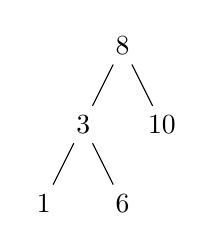
\begin{tikzpicture}[level distance=1cm,
    sibling distance=1cm]
  \node {8}
  child {
    node {3}
    child { node {1} }
    child { node {6} }
  }
  child { node {10} };
\end{tikzpicture}
\end{minipage}
\parbox[b][3.3cm][c]{3em}{\center$\Longrightarrow$}
\begin{minipage}[b][3.3cm][t]{.2\textwidth}
\begin{tikzpicture}[level distance=1cm,
    sibling distance=1cm]
  \node {8}
  child {
    node {3}
    child { node {1} }
    child {
      node {6}
      child { node {4} }
      child { edge from parent[draw=none] }
    }
  }
  child { node {10} };
\end{tikzpicture}
\end{minipage}
\parbox[b][3.3cm][c]{3em}{\center$\Longrightarrow$}
\begin{minipage}[b][3.3cm][t]{.3\textwidth}
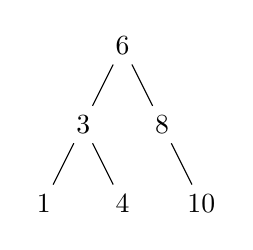
\begin{tikzpicture}[level distance=1cm,
    sibling distance=1cm]
  \node {6}
  child {
    node {3}
    child { node {1} }
    child { node {4} }
  }
  child {
    node {8}
    child { edge from parent[draw=none] }
    child { node {10} }
  };
\end{tikzpicture}
\end{minipage}
\end{center}
A 4-es beszúrása után a 6-os \pr{<} típusú lesz, a
3-as \pr{>} típusú, de probléma csak a legfelső
szinten jelentkezik, ahol a 8-as már eleve \pr{<}
típusú volt. Itt tehát az egész fára fog meghívódni
a forgató \pr{rebalance} operáció, aminek az
eredménye jobboldalt látszik.

\begin{program*}
% del_min_assoc(+Assoc0, ?Key, ?Val, -Assoc)
%                                         [semidet]
del_min_assoc(Tree, Key, Val, NewTree) :-
    del_min_assoc(Tree, Key, Val,
                  NewTree, _DepthChanged).

del_min_assoc(t(Key,Val,_B,t,R), Key, Val,
              R, yes) :- !.
del_min_assoc(t(K,V,B,L,R), Key, Val,
              NewTree, Changed) :-
    del_min_assoc(L, Key, Val, NewL, LeftChanged),
    deladjust(LeftChanged, t(K,V,B,NewL,R),
              left, NewTree, Changed).
\end{program*}
Kitörli a legkisebb kulcsú elemet. \pr{Val} a hozzá
tartozó érték, és az utolsó argumentum a törléssel
keletkezett AVL-fa. Ha a baloldali részfa üres,
akkor a keresett kulcs a gyökérben van, és az új fa
a jobboldali részfa lesz. Egyébként a baloldali
részfában végezzük rekurzívan a törlést, és utána
kiegyensúlyozzuk a \pr{deladjust} szabály
segítségével (ld.~lent).

\begin{program*}
% del_max_assoc(+Assoc0, ?Key, ?Val, -Assoc)
%                                         [semidet]
del_max_assoc(Tree, Key, Val, NewTree) :-
    del_max_assoc(Tree, Key, Val,
                  NewTree, _DepthChanged).

del_max_assoc(t(Key,Val,_B,L,t), Key, Val,
              L, yes) :- !.
del_max_assoc(t(K,V,B,L,R), Key, Val,
              NewTree, Changed) :-
    del_max_assoc(R, Key, Val, NewR, RightChanged),
    deladjust(RightChanged, t(K,V,B,L,NewR),
              right, NewTree, Changed).
\end{program*}
Ugyanez, csak a legnagyobb kulcsú elemmel és
jobboldali rekurzióval.

\begin{program*}
% del_assoc(+Key, +Assoc0, ?Value, -Assoc) [semidet]
del_assoc(Key, A0, Value, A) :-
    delete(A0, Key, Value, A, _).

delete(t(Key,Val,B,L,R), K, V,
       NewTree, WhatHasChanged) :-
    compare(Rel, K, Key),
    delete(Rel, t(Key,Val,B,L,R), K, V,
           NewTree, WhatHasChanged).

delete(=, t(Key,Val,_B,t,R), Key, Val, R, yes) :- !.
delete(=, t(Key,Val,_B,L,t), Key, Val, L, yes) :- !.
delete(=, t(Key,Val,>,L,R), Key, Val,
       NewTree, WhatHasChanged) :-
    del_min_assoc(R, K, V, NewR, RightHasChanged),
    deladjust(RightHasChanged, t(K,V,>,L,NewR),
              right, NewTree, WhatHasChanged),
    !.
delete(=, t(Key,Val,B,L,R), Key, Val,
       NewTree, WhatHasChanged) :-
    del_max_assoc(L, K, V, NewL, LeftHasChanged),
    deladjust(LeftHasChanged, t(K,V,B,NewL,R),
              left, NewTree, WhatHasChanged),
    !.

delete(<, t(Key,Val,B,L,R), K, V,
       NewTree, WhatHasChanged) :-
    delete(L, K, V, NewL, LeftHasChanged),
    deladjust(LeftHasChanged, t(Key,Val,B,NewL,R),
              left, NewTree, WhatHasChanged).
delete(>, t(Key,Val,B,L,R), K, V,
       NewTree, WhatHasChanged) :-
    delete(R, K, V, NewR, RightHasChanged),
    deladjust(RightHasChanged, t(Key,Val,B,L,NewR),
              right, NewTree, WhatHasChanged).
\end{program*}
Általános törlő operáció. Nézzük végig a
\pr{delete/6} egyes eseteit!
\begin{enumerate}
\item Keresett kulcs a gyökérben, baloldali részfa
  üres. Eredmény a jobboldali részfa.
\item Keresett kulcs a gyökérben, jobboldali részfa
  üres. Eredmény a baloldali részfa.
\item Keresett kulcs a gyökérben, és a jobboldali
  részfa mélyebb. Ekkor a jobboldali részfából
  kiveszi a legkisebb kulcsú elemet, és berakja a
  gyökérbe, majd kiegyensúlyozza a fát.
\item Keresett kulcs a gyökérben, és a jobboldali
  részfa nem mélyebb. Ekkor a baloldali részfából
  kiveszi a legnagyobb kulcsú elemet, és berakja a
  gyökérbe, majd kiegyensúlyozza a fát.
\item Keresett kulcs kisebb a gyökér
  kulcsánál. Rekurzív törlés a bal részfában, utána
  kiegyensúlyozás.
\item Keresett kulcs nagyobb a gyökér
  kulcsánál. Rekurzív törlés a jobb részfában, utána
  kiegyensúlyozás.
\end{enumerate}

\begin{program*}
deladjust(no, OldTree, _, OldTree, no).
deladjust(yes, t(Key,Val,B0,L,R), LoR,
          NewTree, RealChange) :-
    deltable(B0, LoR, B1,
             WhatHasChanged, ToBeRebalanced),
    rebalance(ToBeRebalanced, t(Key,Val,B0,L,R), B1,
              NewTree, WhatHasChanged, RealChange).

deltable(-, right, <, no , no ) :- !.
deltable(-, left , >, no , no ) :- !.
deltable(<, right, -, yes, yes) :- !.
deltable(<, left , -, yes, no ) :- !.
deltable(>, right, -, yes, no ) :- !.
deltable(>, left , -, yes, yes) :- !.
\end{program*}
Teljesen hasonló a beszúrás utáni \pr{adjust}
szabályhoz, csak törlés után.

\begin{program*}
rebalance(no, t(K,V,_,L,R), B, t(K,V,B,L,R),
          Changed, Changed).
rebalance(yes, OldTree, _, NewTree,
          _, RealChange) :-
    avl_geq(OldTree, NewTree, RealChange).
\end{program*}
Elérkeztünk az AVL-fák lelkéhez, a forgató
\pr{rebalance} szabályhoz. Az első argumentum azt
mondja meg, hogy szükség van-e forgatásra. Ha ez
\pr{no}, akkor a fa lényegileg nem változik, csak az
egyensúly-szimbólumot állítja be a harmadik
argumentumban kapott értékre (ami a megfelelő
táblázatból lett kiolvasva). Az utolsó argumentum
azt mutatja, hogy a fa mélysége megváltozott-e, és
ha nem történik forgatás, akkor csak átmásolja a
beszúrás/törlés során megállapított értéket.

A tényleges forgatást az \pr{avl\_geq} végzi, aminek
mindössze 3 argumentuma van: a régi fa, a forgatás
után keletkező új fa, és hogy a forgatás során
változott-e a fa mélysége.

\begin{program*}
avl_geq(t(A,VA,>,Alpha,t(B,VB,>,Beta,Gamma)),
        t(B,VB,-,t(A,VA,-,Alpha,Beta),Gamma),
        yes) :- !.
avl_geq(t(A,VA,>,Alpha,t(B,VB,-,Beta,Gamma)),
        t(B,VB,<,t(A,VA,>,Alpha,Beta),Gamma),
        no) :- !.
avl_geq(t(B,VB,<,t(A,VA,<,Alpha,Beta),Gamma),
        t(A,VA,-,Alpha,t(B,VB,-,Beta,Gamma)),
        yes) :- !.
avl_geq(t(B,VB,<,t(A,VA,-,Alpha,Beta),Gamma),
        t(A,VA,>,Alpha,t(B,VB,<,Beta,Gamma)),
        no) :- !.
avl_geq(t(A,VA,>,Alpha,
            t(B,VB,<,t(X,VX,B1,Beta,Gamma),Delta)),
        t(X,VX,-,t(A,VA,B2,Alpha,Beta),
            t(B,VB,B3,Gamma,Delta)),
        yes) :-
    !,
    table2(B1, B2, B3).
avl_geq(t(B,VB,<,
            t(A,VA,>,Alpha,t(X,VX,B1,Beta,Gamma)),
            Delta),
        t(X,VX,-,t(A,VA,B2,Alpha,Beta),
            t(B,VB,B3,Gamma,Delta)),
        yes) :-
    !,
    table2(B1, B2, B3).

table2(< ,- ,> ).
table2(> ,< ,- ).
table2(- ,- ,- ).
\end{program*}
Nézzük végig az egyes eseteket!
\begin{enumerate}
\item \pr{>/>}: a jobboldali részfa túl mély, és
  annak a jobboldali részfája a mélyebb. A forgatás
  hatására a mélység csökken.
\begin{center}
\begin{minipage}[b][2.5cm][t]{.3\textwidth}
\begin{tikzpicture}[level distance=1cm]
  \node {A}
  child { node {$\alpha$} }
  child {
    node {B}
    child { node {$\beta$} }
    child { node {$\gamma$} }
  };
\end{tikzpicture}
\end{minipage}
\parbox[b][3cm][c]{2.5em}{\center$\Longrightarrow$}
\begin{minipage}[b][2.5cm][t]{.3\textwidth}
\begin{tikzpicture}[level distance=1cm]
  \node {B}
  child {
    node {A}
    child { node {$\alpha$} }
    child { node {$\beta$} }
  }
  child { node {$\gamma$} };
\end{tikzpicture}
\end{minipage}
\end{center}
\item \pr{>/-}: a jobboldali részfa túl mély, és az
  egyensúlyban van. Ez csak baloldali törlés után
  jöhet létre. A forgatás megegyezik az előzővel, de
  ilyenkor a mélység nem változik.
\item \pr{</<}: az 1-es tükrözve.
\item \pr{</-}: a 2-es tükrözve.
\item \pr{>/<}: a jobboldali részfa túl mély, és
  annak a baloldali részfája a mélyebb. A forgatás
  hatására a mélység csökken. Az \pr{A}-nál és
  \pr{B}-nél levő egyensúly-szimbólumokat az
  \pr{X}-nél levő alapján a \pr{table2} táblázat
  adja meg.
\begin{center}
\begin{minipage}[b][3.5cm][t]{.25\textwidth}
\begin{tikzpicture}[level distance=1cm]
  \node {A}
  child { node {$\alpha$} }
  child {
    node {B}
    child {
      node {X}
      child { node {$\beta$} }
      child { node {$\gamma$} }
    }
    child { node {$\delta$} }
  };
\end{tikzpicture}
\end{minipage}
\parbox[b][3cm][c]{3.5em}{\center$\Longrightarrow$}
\begin{minipage}[b][3.5cm][t]{.45\textwidth}
\begin{tikzpicture}[level distance=1cm,
    level 1/.style={sibling distance=2.5cm},
    level 2/.style={sibling distance=1.5cm}]
  \node {X}
  child {
    node {A}
    child { node {$\alpha$} }
    child { node {$\beta$} }
  }
  child {
    node {B}
    child { node {$\gamma$} }
    child { node {$\delta$} }
  };
\end{tikzpicture}
\end{minipage}
\end{center}
\item \pr{</>}: az 5-ös tükrözve (ilyen volt a fenti
  beszúrásos példa).
\end{enumerate}

Itt érdemes megjegyezni, hogy a mélységcsökkenést
jelző utolsó argumentumot csak a \pr{deladjust}
veszi figyelembe, az \pr{adjust} nem. Ennek az az
oka, hogy ha beszúráskor nőne a mélység, akkor a
forgatás azt mindig kompenzálja, tehát végül az
eredeti állapothoz képest a mélység nem
változik. Ezzel szemben törlésnél ha forgatásra van
szükség, akkor csak ettől függ, hogy a mélység
csökken-e.

Ezzel vége a könyvtár forráskódjának. Ez egy szép,
jól érthető program, ami kevés külső definíciót
használ, ugyanakkor rendkívül tanulságos.

\section{Projekt: prioritásos sor}
Egy másik gyakran szükséges adatszerkezet a
\emph{prioritásos sor}, amiben minden elemhez egy
prioritást rendelünk, és mindig a legmagasabb
prioritásút vesszük ki belőle. A következő
szabályokkal kezelhető:
\begin{itemize}
\item \pr{üres\_sor(?Sor)} [semidet]
\item \pr{sorba\_tesz(+Sor, +Prioritás, ?Elem, -Sor1)} [det]
\item \pr{maximum\_elem(+Sor, ?Elem)} [semidet]
\item \pr{maximumot\_kivesz(+Sor, -Prioritás, ?Elem, -Sor1)} [semidet]
\end{itemize}
A kényelmes használat kedvéért még érdemes
listából/listává átváltó szabáyokat is készíteni
(ahol a lista \pr{Prioritás-Elem} párokból áll):
\begin{itemize}
\item \pr{listából\_sor(+Lista, -Sor)} [det]
\item \pr{sorból\_lista(+Sor, -Lista)} [det]
\end{itemize}
Ennek egy egyszerű megoldása az, hogy a betevés
sorrendjében egy listában tároljuk az elemeket --
ebben az esetben a maximum megkeresése ill. a sorból
kivétel $O(n)$ műveletigényű lesz. Egy másik
lehetőség, hogy az elemeket mindig csökkenő
sorrendben tároljuk; ekkor az új elem betevése lesz
$O(n)$-es komplexitású.

Egy hatékonyabb módszert kapunk, ha itt is egy fát
használunk. Ebben a fában a csúcsokból nem csak
kettő, hanem több ág is indulhat, és csak azt várjuk
el, hogy a csúcsban levő prioritás legalább akkora
legyen, mint az alatta levő részfák maximum
prioritása, így a maximum mindig a gyökérben
lesz. Ezt ,,párosító kupacnak'' nevezik.
\index{kupac!párosító}

Két ilyen fa egybeolvasztása nagyon egyszerű:
megnézzük, hogy melyik gyökerének nagyobb a
prioritása, és az marad a gyökér, a másik pedig ez
alá kerül új részfaként. A beszúrás is ennek egy
speciális esete, ahol a beszúrt elem egy olyan fa,
aminek csak gyökere van.

Az egyetlen bonyolultabb -- $O(\log n)$ komplexitású
-- művelet a maximális prioritású elem
kivétele. Ilyenkor az összes alatta levő részfát
egybe kell olvasztani, amíg csak egy nem marad. Ez
sokféleképp megtehető, és a különböző módszerek más
jellegű fákat eredményeznek. A klasszikus megoldás
az, hogy a részfákat először balról jobbra páronként
egybeolvasztjuk (innen a nevében a \emph{párosító}),
és utána a jobboldalitól elindulva a már
egybeolvasztott párokat egyenként
hozzáolvasztjuk. (Ez rekurzív módon nagyon
egyszerűen megfogalmazható.)

Nézzünk egy példát! Jelölje \pr{P-[P1,P2,..,Pn]} azt
a fát, aminek a gyökerében \pr{P}, az alatta levő
részfák gyökerében pedig \pr{Pi} prioritások vannak
(a további, érdektelen részfákat \pr{..} jelöli):
\begin{query}
10-[5,8,2,8,10,1,3]
\end{query}
Maximumkivétel $\Rightarrow$ 7 különálló fa:
\begin{query}
5-[..] 8-[..] 2-[..] 8-[..] 10-[..] 1-[..] 3-[..]
\end{query}
Párosítás balról jobbra $\Rightarrow$ 4 különálló
fa:
\begin{query}
8-[5,..] 8-[2,..] 10-[1,..] 3-[..]
\end{query}
Egyesítés jobbról balra, amíg csak 1 marad:
\begin{query}
8-[5,..] 8-[2,..] 10-[3,1,..]

8-[5,..] 10-[8-[2,..],3,1,..]

10-[8-[5,..],8-[2,..],3,1,..]
\end{query}
\begin{problem}
Készíts egy prioritásos sor adatszerkezetet párosító
kupaccal!
\end{problem}
